\chapter{Introduction}

	Our Universe's origin has always been a mystery until the last century when humankind started looking for answers to the unanswered questions about the evolution of the Universe. The process of finding solutions to problems that arose built up to a field of study called cosmology. This field has drastically impacted our knowledge of the universe evolution~\citep{book:909085}. The primordial humankind assumed that the Sun, the moon, and other planets orbited the Earth until Nicolaus Copernicus and other astronomers replaced the geocentric model with the heliocentric model~\citep{sep-copernicus, kanas}.
	
	The celestial mechanics area of study came into existence after Isaac Newton made discoveries that the elliptic planet motion, among other things, can be explained by gravitational force attraction. He also reasoned that the Kepler ellipse is only an approximation of planetary motion's true nature (interaction between planets)~\citep{crowe2013theories,sep-copernicus}. In the modern study of the Universe, Albert Einstein has been a significant influence on the theory of general relativity, which presents the mathematical framework required to explain the evolution of the universe~\citep{1965ApJ...142..419P}.
	
	As a result of all these findings, Georges Lemaitre proposed the Big Bang theory, the contemporary model that provides a complete explanation of the Universe expansion~\citep{1926ApJ....64..321H}. The Big Bang theory was established from Hubble's law and subsequently by Arno Penzias and Robert Wilson in 1964 from discovering the cosmic microwave background (CMB)~\citep{1965ApJ...142..419P,2003RvMP...75..559P,1929PNAS...15..168H}. The Supernova Cosmology Project and the High-Z Supernovae Search Team in 1998 uncovered the acceleration of the Universe. They used type Ia supernovae to determine the acceleration of the Universe~\citep{1998AJ....116.1009R, 1999ApJ...517..565P}. The Universes expansion acceleration is described by the dark energy that accounts for approximately 74 percent of the Universe's energy density. Today, any dark energy discoveries are still as disconcerting in the study of astrophysics and particle physics~\citep{2008ARA&A..46..385F}.\\
	
	\section{History of the Universe}
	
	\autoref{Fig:timeline} shows the cosmic history of the Universe, where the earliest era was the Planck era. The earliest era is from zero to \SI{e-43}{s} from the birth of the Universe. What happened before the Planck era is unknown to physicists; the only progress made was to build up from what was known from the birth of the Universe. Quantum theory of gravity provides the background to understand what happened before this time~\citep{1981PhRvD..23..347G}. What was deduced from the Planck era was the Universe's rapid exponential expansion, governed by the Epoch of Inflation. It is \SI{e-34}{s} from the birth of the Universe~\citep{Planck}.
	
	\begin{figure}
		\begin{center}
			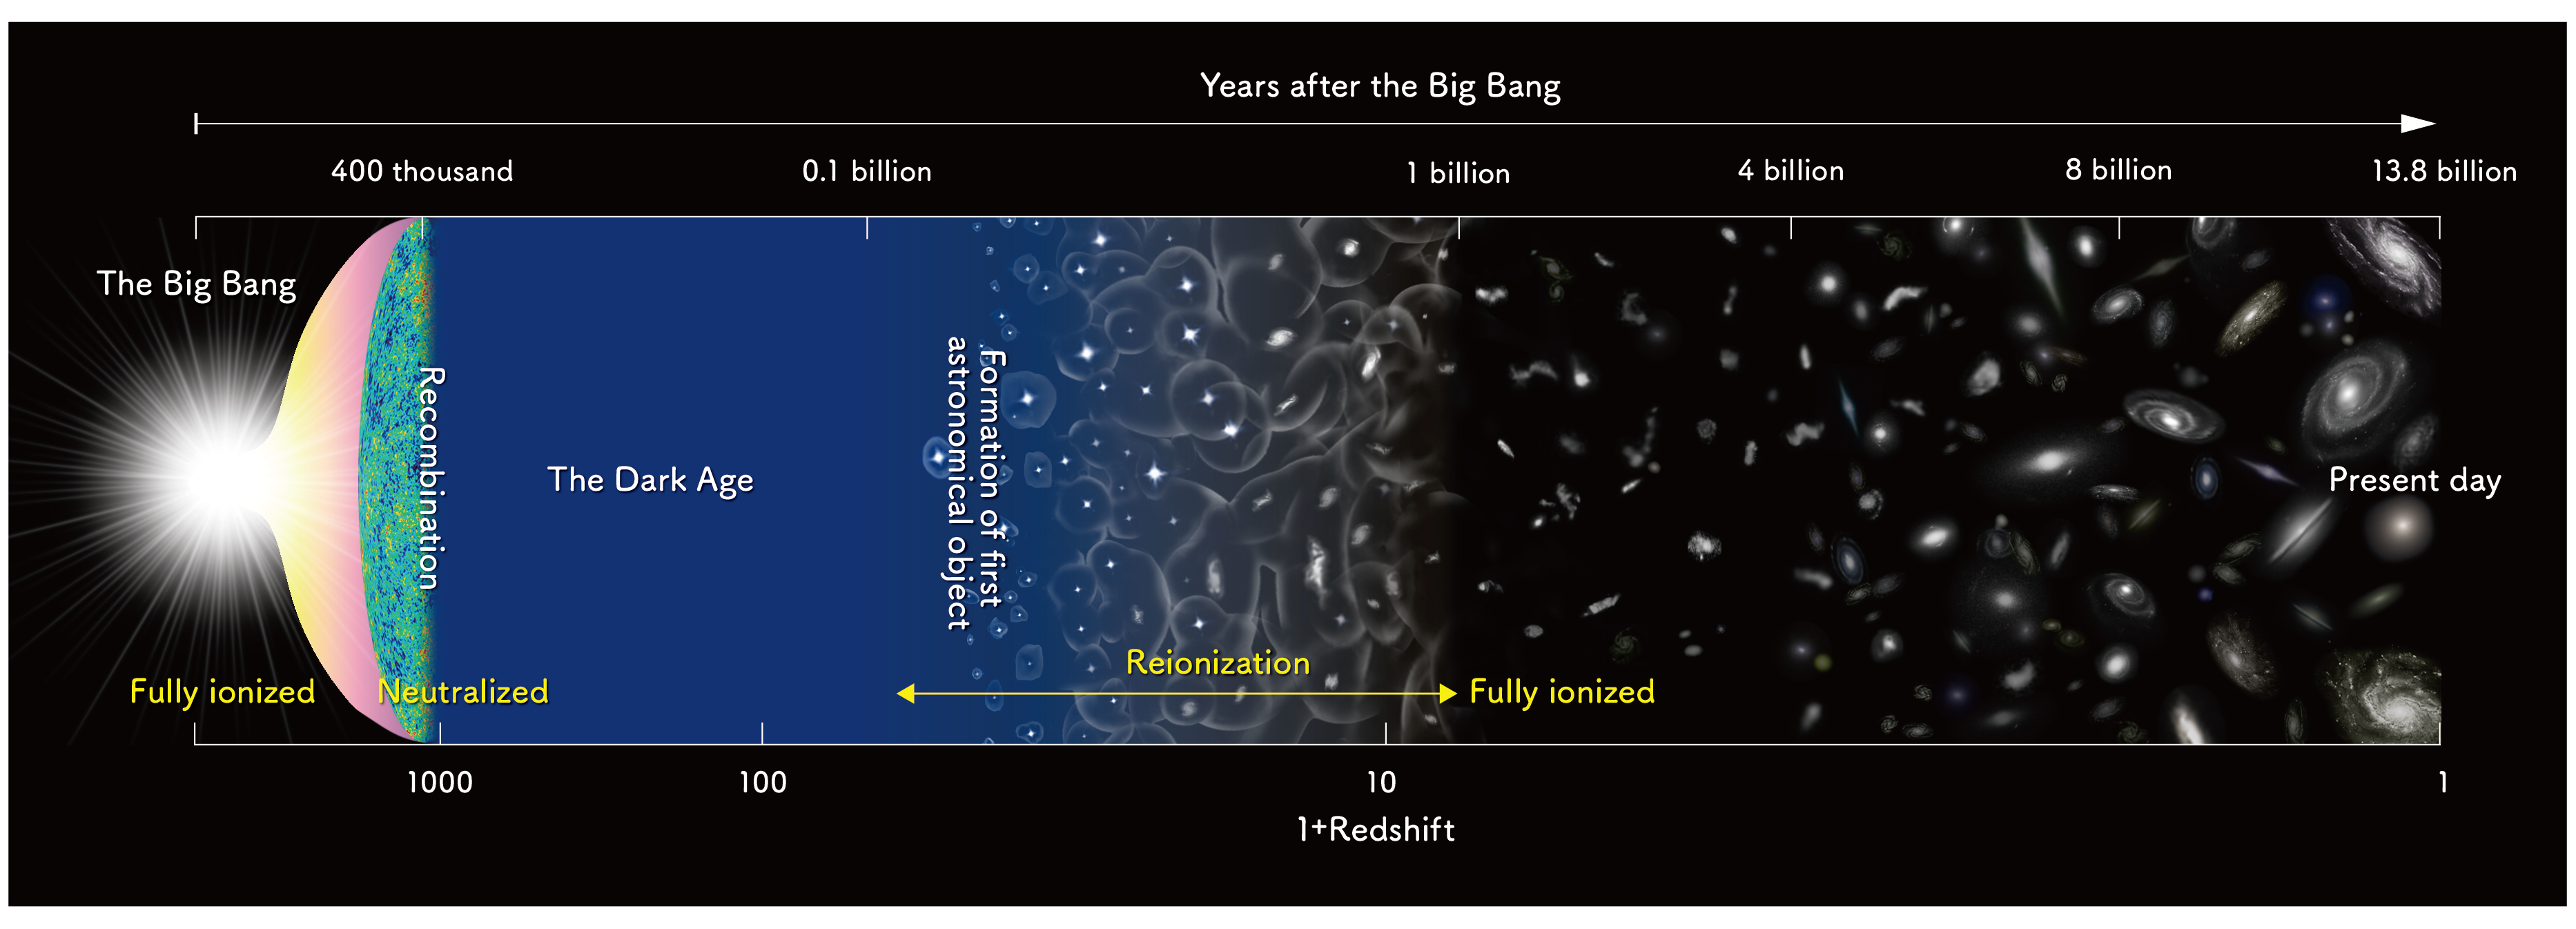
\includegraphics[width=\linewidth]{Figures/Reionizationtimeline.jpg}
			\caption{The cosmic history of the Universe from the Big Bang to its early years, through the dark ages to the epoch of reionization and the post-reionization epoch. Image credit:National Optical Astronomy Observatory}
			\label{Fig:timeline}
		\end{center}
	\end{figure}
	
	Recombination occurred when the neutral hydrogen (HI) was formed from the cool enough Universe at a redshift of z $\sim1100$. The redshift-wavelength relation is mathematically presented by
	\begin{equation}
	\begin{split}
	1+z & = \frac{\lambda_{obs}}{\lambda_{emit}}= \frac{1}{a}
	\end{split}
	\end{equation}
	where $z$ is the redshift, $\lambda_{obs}$ is the wavelength of the observed signal, $\lambda_{emit}$ is the wavelength of the signal emitted, and $a$ is the Universe expansion scale factor.
	
	Before that, electrons were not bound to protons, and the Universe contained ionized plasma known as photon-baryon fluid. Decoupled photons then formed the CMB. The first instance of the CMB was observed by~\citep{1965ApJ...142..419P} after the era of recombination. 
%	The telescopes that braced the Big Bang theory were the Cosmic Background Explorer (COBE)~\citep{2004astro.ph..2528M}. 
	Subsequently, the HI became the dominant baryonic component of the intergalactic medium (IGM) before the first stars' formation during the dark ages ($1100 \gtrsim z \gtrsim 30$). There was rapid cooling of gas relative to the CMB. If the hydrogen can be mapped in this era, valuable cosmological data can be produced~\citep{11, 2004PhRvL..92u1301L}.\\
	
	There were density fluctuations in the distribution of matter, and the overdense regions collapsed under the influence of gravity, ultimately creating the first stars. Thus, nuclear reaction resulted in Cosmic Dawn ($30\gtrsim z \gtrsim 10$). An enormous emitted energy from the stars reionizes the Universe causing ionization. This further results in stars exploding due to gravitational disintegration leading to the formation of galaxies. There is a decelerating effect in the Universe expansion due to gravity's force within dominating matter~\citep{2017arXiv170808521D, 2012AdSpR..49..433B}.\\
	
	Throughout the cosmological epochs, what is known is minimal because it is challenging to observe them directly. Nevertheless, the new occurrence of \SI{21}{cm} cosmology has imparted the capability of bridging the gap between what is known and what is not know about the eras of our history~\citep{2014ApJ...782L...9V, 2013PhRvD..87d3002L}. A brief overview of the history of the Universe has been given, and the next section will cover the 21 cm cosmology, dark ages, and cosmic dawn in more detail.
	           
	\section{Cosmology with Redshifted 21-cm Emission}
	
	\attention{[This section needs to appear before you talk about the details of $\delta T_b$.  The reader won't be able to understand $\delta T_b$ if you haven't introduced 21-cm emission!]}
	
	%	\textcolor{red}{High redshift observations of the globally averaged 21-cm emission of neutral hydrogen has been recently proposed as a window into the cosmic dawn, an epoch of cosmic evolution that occured roughly a few hundred million years after the big bang, when the first stars ignited in the universe~\citep{2012RPPh...75h6901P}.\\}
		
	Observations of redshifted 21 cm line of neutral hydrogen at radio frequencies are a rapidly growing area of cosmology research that can potentially shed light on numerous epochs in the Universe's history~\citep{2012RPPh...75h6901P}.
	
	Our Universe is rich in hydrogen gas, hence a
	concerted effort in the experimental community to develop telescopes for mapping neutral hydrogen via \SI{21}{cm} emission wavelength line. The \SI{21}{cm} wavelength of hydrogen gas is being observed by several experiments that are modeled for Hydrogen mapping in our Universe. This hydrogen line is an essential mechanism as it helps in probing the dark ages to the epoch of reionization (EoR)~\citep{2013PhRvD..87d3002L,2014ApJ...782...66P}. The generation of the hydrogen line (\SI{21}{cm} line or HI line) is due to the intrinsic spin of the hydrogen atoms, namely, an electron and the proton~\citep{book:832129}.\\
	
	The electron and proton spins can be oriented in either the opposing or the same direction respective to each other. When they are in an opposing direction, they result in an antiparallel spin, which implies that the hydrogen atom is in the lower energy state. When they are in the same direction, they result in a parallel spin, which implies that the hydrogen atom is in a higher energy state. Once an electron transition from one state to another, the hydrogen atom discharges a photon with a \SI{21}{cm} wavelength equivalent to (\SI{1420}{MHz}). The hyperfine splitting of the two energy states equivalent to \(\Delta E =  5.9 \times 10^{-6} \ eV\) is a consequence of the dissimilarity between the spin states.
	\autoref{Fig:21cm} shows the spin-flip transition process~\citep{16, book:832129}.
	
	\begin{figure}
		\begin{center}
			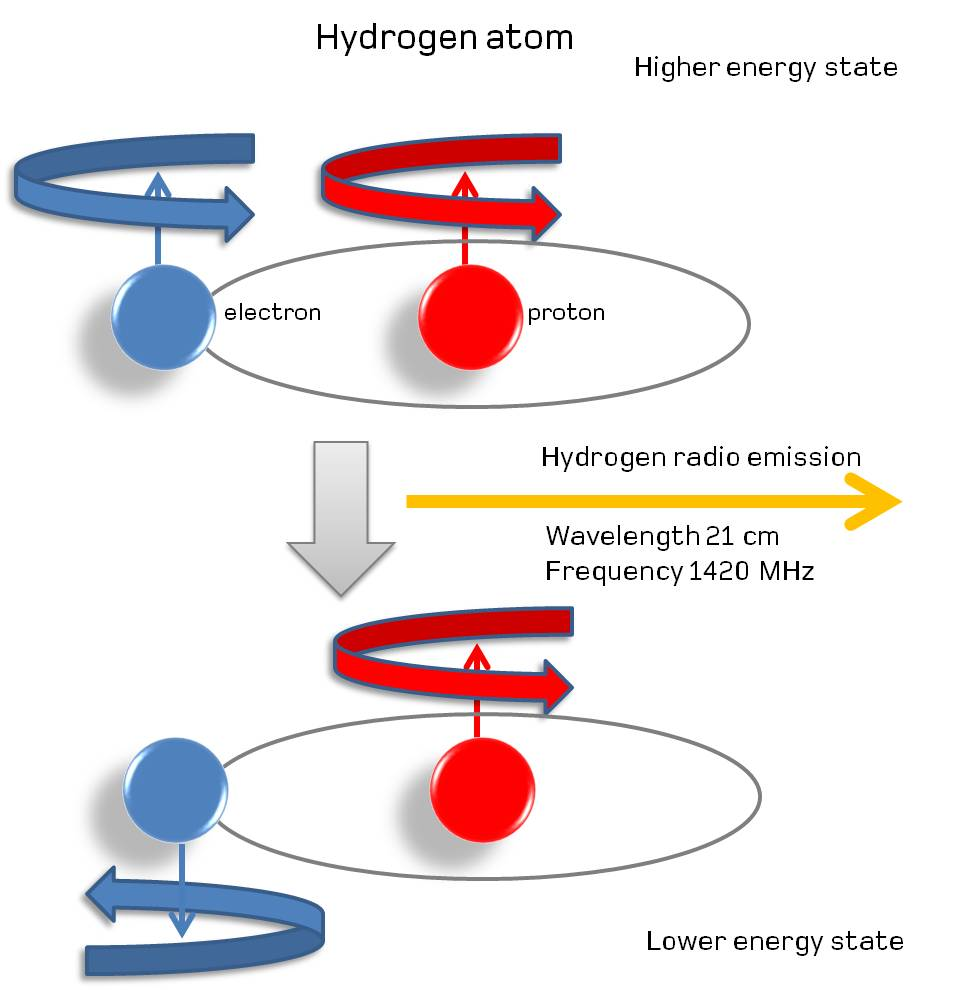
\includegraphics[width=0.5\linewidth]{Figures/Hydrogenemission1.jpeg}
			\caption{The formation of the \SI{21}{cm} wavelength line by the process of spin flip transition where the hydrogen atom moves from one energy state to another. Image credit: {Square Kilometre Array}.}
			\label{Fig:21cm}
		\end{center}
	\end{figure}
	
	$n_0$ and $n_1$ are the two relative spin states that define the spin temperature $T_s$ using the relation,
	
	\begin{equation}
	\frac{n_0}{n_1} = \frac{g_1}{g_0}e^{(-E_10)/{k_B}{T_s}} = 3e^{{-T_*}{T_s}}
	\end{equation}
	
	where $\frac{g_1}{g_0}/$ = 3 is the spin degeneracy of the triplet and singlet levels, $T_s$ is the spin temperature, which is the excitation temperature of the 21 cm hydrogen line, and $T_{*}$ $\equiv$ hc/k $\lambda_{21cm}$ = 0.068 K which is the equivalent temperature of the hyperfine splitting of the two energy levels between the two states~\citep{2012RPPh...75h6901P}.
	
	\begin{figure}
		\begin{center}
			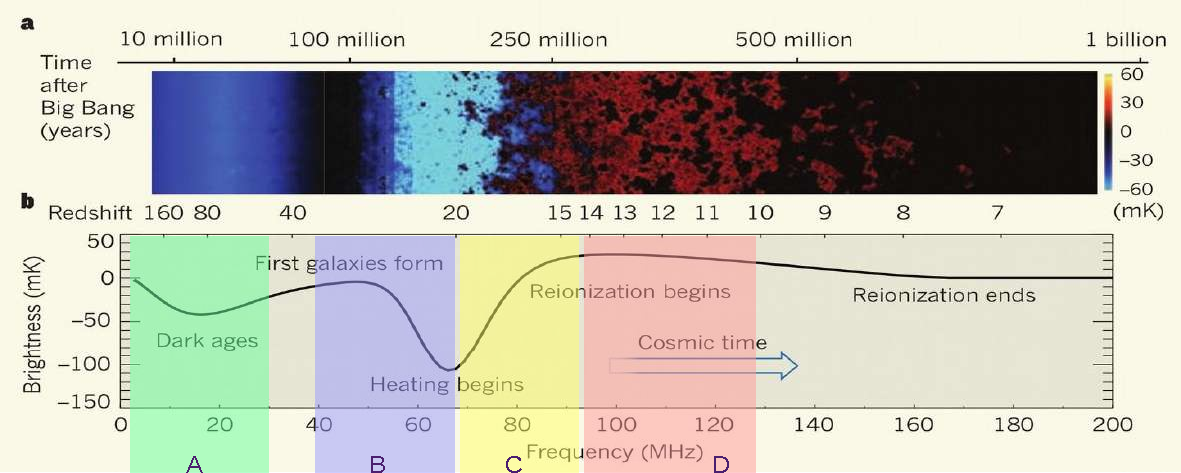
\includegraphics[width=\linewidth]{Figures/epo.pdf}\\
			\caption{Frequency structure of the globally averaged 21 cm signal, (a) shows two dimensional slice of the time evolution of the 21 cm brightness temperature and (b) shows predicted time evolution of the global 21 cm brightness temperature with relevant epochs~\citep{2012RPPh...75h6901P}. There are different physical processes that govern the four highlighted (A to D) periods and the details are discussed in the main text}.
			\label{Fig:epochs}
		\end{center}
	\end{figure}
	
	\subsection{Dark Ages}
	
	The cosmic dark ages lie between recombination and cosmic dawn, beginning $\sim380,000$ years after the big bang and ending a few tens of million years later ($1100 > z > 30$),~\citep{2014arXiv1412.2096J} during which there were no luminous sources. The cosmic dark ages possess distinctive features that have never been explored to date. 
	
	
	The 21 cm brightness temperature relative to CMB ($\delta$$T_b$), which provides a source of external 21 cm radiation, depends on the three sources, namely the kinetic gas temperature, $T_K$, which characterizes the thermal motion of atoms in the gas, the hydrogen spin temperature ($T_S$) which is the excitation temperature of the 21 cm line, and the coupling between $T_S$ and $T_K$ (which arises from different mechanisms)~\citep{2015aska.confE...1K,2006PhR...433..181F}. The equation  
	
	\begin{equation}
	\delta{T_b}\propto {x_{HI}}(1+z)^{1/2}({T_s}-{T_{CMB}})/{T_s}
	\end{equation}
	
	relates $\delta$$T_b$ to important factors which are \(x_{HI}\), the fraction of neutral hydrogen, redshift ($z$) and two temperatures, the spin temperature ($T_s$) and the CMB temperature ($T_{CMB}$).
	
	\attention{[In the sections below, refer to the labeled periods in Figure~\ref{Fig:epochs} to guide your discussion.]} \\
	
	Figure~\ref{Fig:epochs} describes the physical processes that are responsible for the frequency structures we see in the evolution of the sky-averaged 21 cm brightness temperature. Region A highlighted in green explains the period where the free electrons were no longer present. During this epoch right after recombination $T_K$=$T_\gamma$=$T_S$ where $T_\gamma$ is the temperature of the neighbouring bath of radio photons, typically set by the CMB so that $T_\gamma$ = $T_{CMB}$. During this period, matter that had separated from the CMB was cooled adiabatically as the Universe expanded, which led to $T_K$ decreasing below $T_\gamma$~\citep{2006PhR...433..181F}. The CMB flux must have been resonantly absorbed by the cosmic neutral hydrogen through its spin-flip 21 cm transition before the first stars formed. $T_S$ is coupled to $T_K$ as the collision between hydrogen atoms becomes initially effective, resulting in $\delta T_b$ decreasing initially. As the Universe expands and collisional coupling becomes ineffective, $T_S$ reverts to $T_\gamma$ because of CMB absorption.
	
	At this juncture, the most dominating matter in the Universe was the dark matter and meager amounts of ordinary matter (neutral hydrogen and helium). After a few hundred million years, the dark matter which was predominant started to collapse into halo-like structures through gravitational collapse, steadily cumulating physical matter and finally forming the first stars and galaxies, and that was the end of the cosmic dark ages~\citep{2003Sci...300.1904M}.
	
%	\begin{figure}
%		\begin{center}
%			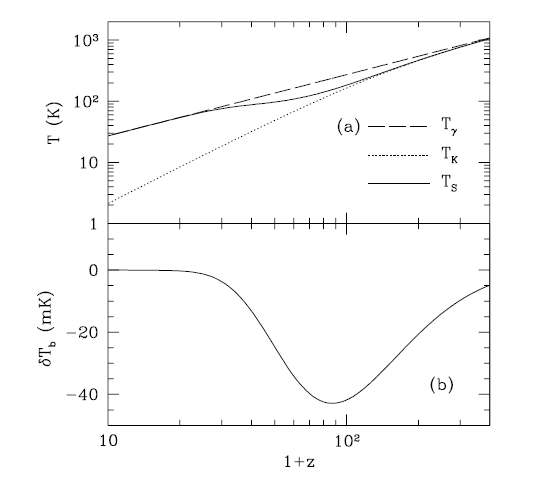
\includegraphics[width=0.7\linewidth]{Figures/DA.png}\\
%			\caption{(a) Plot of $T_S$, $T_\gamma$, and $T_K$ during the dark ages, as calculated from initial conditions given by the CMB and (b) $\delta$$T_b$ during the same period with only collisional coupling present. Plots taken from~\citep{2006PhR...433..181F}} 
%			\label{Fig:DA}
%		\end{center}
%	\end{figure}
	
	\subsection{Cosmic Dawn}
	    
	    After the first stars' formation, their UV radiation couples to the HI line through the Wouthuysen-Field effect. The formation of the frequency structure results from the emission of Lyman Alpha photons by the first stars, strongly coupling the $T_K$ and $T_S$ of the IGM via the WouthuysenField effect (WF); the described period is shown in Region B highlighted in purple. At the first stars' birth, the WF sets the $ T_K $ and $ T_S $ equal, leading to a drastic absorption feature~\citep{2014ApJ...782L...9V}. The significant absorption HI feature is created by this coupling, which can be used to probe the first stars' spectra, with the potential of differentiating between Pop II and Pop III stars. Region C highlighted in yellow shows a period where the X-rays are emitted by hot accretion disks around the first stellar remnants (e.g., black holes) that effectively heat the cold HI gas (The gas surrounding these stars was both radiated and heated. By the Wouthuysen-Field (W-F) effect, the cold gas temperature was coupled from the spin-temperature. The second period (the cosmic dawn) \attention{["cosmic dawn" starts with the absorption feature; refer to the labels in Figure~\ref{Fig:epochs} to guide your discussion]} originated where the hydrogen line was seen in absorption. As the stars continued to form, it is believed that there was an appearance of the first X-ray emitting sources, heating the neutral gas and thereby (again via the W-F effect) raising the overall spin-temperature to higher than the CMB temperature.\\
	    
	    
	    Consequently, the 21-cm line became visible in emission at $z\sim15$. During radiation and heating, these first sources (possibly including mini-quasars) also ionized the gas around them, and a period of reionization started that is thought to have lasted until $z\sim5~to\sim 6$~\citep{2015aska.confE...1K}). During the period shown by Region D highlighted in red, the HI feature observations are sensitive to the black hole's properties and the progenitor's metallicity, offering further insight into first-star formation.~\citep{11}. When reionization begins, the neutral hydrogen supply is depleted ($x_{HI}$ decreases to zero), so $\delta T_b$ eventually also flatlines to zero because there is no more 21 cm signal left. \\ 
	    
	    \section{Hydrogen Line Observational Challenges}
	    
	    \attention{[These observational sections can stay here, after the discussion of $\delta T_b$.  Only the introduction about the hyperfine transition should be moved earlier.]}
	    
	    Since our Universe is rich in hydrogen, and the long-wavelength radiation can penetrate dust, this \SI{21}{cm} radiation is an ideal tool for probing the history of the Universe at any epoch of interest. However, the ground-based telescopes and experiments are faced with a challenge when it comes to using the \SI{21}{cm} highly redshifted line emission to observe the dark ages, cosmic dawn, and the Epoch of Reionization~\citep{2016ExA....41..271R}. The challenges are namely human-made Radio Frequency Interference (RFI), foregrounds, ionospheric interferences, and the instrumental systematics, which is non-transparent below \SI{10}{MHz}. 
	    
	    \subsection*{Brightness of Foreground Emission}
	    
	    The	primary challenge is the extreme brightness of foreground emission, contributed by both Galactic and extragalactic sources.
	    The brightness temperatures of the foreground emission are 4-5 orders of magnitude brighter than the brightness temperature of the cosmological \SI{21}{cm} signal, which is $\sim$ 0.14 mK at $z\sim0.8$~\citep{2018RAA....18..114H}.
	    
	    The Galactic synchrotron emission is primarily included in the foregrounds at low frequency, which originated from the cosmic ray electrons' movement in the Galactic magnetic field. Free electrons scattering off ions without being captured produces the Galactic free-free emission. The extragalactic foregrounds are predominantly radio-loud galaxies and quasars~\citep{2018RAA....18..114H, 2008MNRAS.389.1319J}.
	    
	    \subsection*{Instrumental Systematics}
	    
	    There needs to be a precise calibration of instrumental systematics to remove instrument effects from the data.
	    
	    Instrumental systematics further complicate this effort, causing foreground signal to contaminate Fourier modes in the data that would otherwise only be noise limited. Instrumental systematics have limited many of the current upper limits on the 21 cm power spectrum. Therefore, precise modeling and separation of instrumental systematics will likely be necessary for second-generation 21 cm observations to make sturdy observations of the 21 cm cosmological signal. Instrumental systematics includes calibration errors, ionospheric faraday rotation, primary beam ellipticity, analog signal chain imperfections (such as impedance mismatches), internal instrument couplings, such as signal chain reflections, and antenna cross-coupling (i.e., crosstalk)~\citep{2020ApJ...888...70K}.
	    
	    
	    
	    \subsection*{RFI}
	    
	    Besides astrophysical challenges, human-made RFI saturates the frequency bands, increasing the need for isolated remote deployment sites. 
	    
	    The brightness of the RFI on the 21 cm observations can have up to orders of magnitude beyond the Galactic and extragalactic foregrounds. Unfortunately, RFI introduces a reduction in sensitivity in two separate but distinct ways: direct contamination by having similar spectral characteristics and overpowering the 21cm signal. The other is the introduction of a complex sampling function due to missing data. This produces correlations between modes when computing the Fourier transform along the frequency axis (Offringa et al. 2019). Therefore,  identifying RFI while not falsely identifying non-RFI as RFI is crucial, further complicating our sampling function over frequency~\citep{2019MNRAS.488.2605K}.
	    
	    \subsection*{Ionospheric Contamination}
	    
	    The Earth's ionosphere also introduces significant fluctuations, which becomes increasingly refractive and turbulent below 100 MHz and becomes practically opaque below 10 MHz. Also, "filled aperture" antennas (typically paraboloidal reflectors), commonly used as interferometer elements at higher frequencies, become impractically large below 100 MHz; therefore, beamforming arrays consisting of many low-gain elements must be used instead. Examples of such arrays include the 22-MHz narrowband dipole array at Penticton, British Columbia, active during the 1960s~\citep{2005ITAP...53.2480E}.\\
	    
	    
	    In order to minimize RFI and ionospheric contamination, there have been proposals to observe long wavelengths from space-based telescopes further away from the ionosphere of our planet. These space-based telescopes do not exist yet, and there are several ground-based experimental efforts to understand how well we can make measurements from Earth~\citep{2016ExA....41..271R}. \\
	    
	    \section{Previous Cosmic Dawn and Low-frequency Experiments}
	    
	    Even with the challenges that are encountered in doing the 21 cm cosmology, several experiments nevertheless use the \SI{21}{cm} hydrogen line to study the evolution of the Universe. These experiments are aimed at observing different epochs of the Universe including dark ages (z $\sim1100$ - z $\sim30$), cosmic dawn (z $\sim30$ - z $\sim10$) and epoch of reionization (z $\sim10$ - z $\sim2.5$). Some of the ongoing global 21 cm experiments are discussed in the following subsections.\\
	    
	    %	\textcolor{red}{EDGES, SARAS2, LEDA, CTP, Bighorns, etc}
	    
	    \subsection{Global Signal Experiments for Cosmic Dawn}
	    
	    The Experiment to Detect the Global EoR Signature (EDGES) is located at Murchison Radio-astronomy Observatory (MRO) in Western Australia. The goal of the project is radio detection of characteristic hydrogen signatures from cosmic dawn and the epoch of reionization. EDGES consists of a high-band instrument operating over the 90-200 MHz (14 $>$ z $>$ 6) range, a mid-band instrument operating over 60–160 MHz, and a low-band instrument that is sensitive to the 50-100 MHz (27 $>$ z $>$ 13) range~\cite{2017ApJ...835...49M}.\\
	    
	    The Large aperture Experiment to Detect the Dark Ages (LEDA) experiment operates as part of the Long Wavelength Array at the Owens Valley Radio Observatory (LWA-OVRO). The LWA-OVRO array consists of 251 dual-polarized dipole antennas in a \SI{100}{\meter} radius circle and five outrigger antennas were fitted with LEDA instrumentation. LEDA operates in the frequency range 10–88 MHz. The instrumentation of LEDA facilitates \textit{in situ} characterization of the foreground, monitoring the ionosphere, and measuring antenna gain patterns during observations~\citep{2012JAI.....150004T, 2018MNRAS.478.4193P}.\\
	    
	    Broadband Instrument for Global HydrOgen ReioNisation Signal
	    (BIGHORNS) is a portable, low power consuming total-power radiometer deployed in remote, radio-quiet locations in Western Australia. The experiment uses an off-the-shelf biconical antenna, oriented East-West, and placed at the height of 52 cm on a 3 m x 3 m ground screen. Over the 2012–2014 season, BIGHORNS collected data from three Western Australia locations – Muresk; Eyre Bird Observatory (EBO); and Wondinong Station. Based on test data collected using the prototype system, BIGHORNS made several improvements in the instrument, namely, the addition of a hot/cold load calibration scheme, replacing solid-state switches with mechanical switches in the front end in order to eliminate unwanted attenuation, removal of the 3 dB attenuator between the antenna and the LNA, and replacing the biconical antenna with a conical log spiral antenna which is better matched over a wide frequency band. Most of these improvements are believed to improve calibration accuracy significantly~\citep{2015PASA...32....4S}.
	    
	    \subsection{Imaging below 30 MHz}
	    
	    {\bf{Long Wavelength Astronomy Background}}\\
	    
	    The father of radio astronomy, Karl G. Jansky, played a massive role in the inauguration of radio astronomy dating back to 1931. At that time, he was an employee at the Bell Telephone Laboratories as a radio engineer. Jansky was allocated to study and solve the problem that hindered the radio communication systems. Using highly directive antenna arrays shown in \autoref{Fig:Jansky}, he discovered that the static caused the radio frequency noise that hindered the communication systems from thunderstorms~\citep{book:BasicsofRA, book:RA}.\\
	    
	    \begin{figure}
	    	\begin{center}
	    		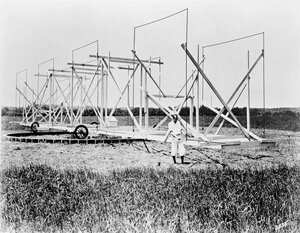
\includegraphics[width=0.7\linewidth]{Figures/jansky1.jpg}
	    		\caption{Jansky's highly directive antenna arrays which he used to discover the cause of RFI that hindered the communication systems at Bell Telephone Laboratories~\citep{book:BasicsofRA}}.
	    		\label{Fig:Jansky}
	    	\end{center}
	    \end{figure}
	    
	    The antenna that he constructed operated at an approximated frequency of \SI{20}{MHz}, corresponding to an approximate long wavelength of \SI{15}{m}. He further found radio radiation from the Galactic Center at the operating frequency. Out of interest in Jansky's instigating discoveries, Grote Reber designed a radio telescope that operated at a range of approximately \SI{10}{MHz} to \SI{160}{MHz} (\SI{30}{m}-\SI{2}{m} wavelength) in 1937. He discovered that the authoritative source at longer wavelengths was the Milky Way area. Furthermore, he realized that the radio telescope acts like a bolometer or a device to measure the heat. The antenna's radiation resistance measures an equivalent temperature of a distant part of space to which the 24 antenna response pattern projects it~\citep{1988JRASC..82...93R, CosmicStatic,2012PASP..124.1090H}.
	    
	    Because of the research done for the communication systems, radio astronomy was born and expanded to radio astronomy and astrophysics~\citep{2012PASP..124.1090H}. The hydrogen line research area had an accelerated discovery, which was allocated an operating frequency of \SI{1420}{MHz} (\SI{21}{cm} wavelength) ~\citep{10.2307/530765}. After all these discoveries, the long-wavelength astronomy fascination has been resuscitated in the present epoch.\\
	    
	    {\bf{Long Wavelength Astronomy Experiments}}\\
	    
	    There are quite a few low-frequency experiments, but this document will briefly discuss a few measurements that exist at $\lessapprox$ 30 MHz. Two of these experiments represent the lowest frequencies measured to date (Reber's antenna, RAE-B). The other two represent the highest resolutions achieved in this frequency range (DRAO, OVRO-LWA).\\
	    %	    
	    %	    {\bf LWA:} It is based in New Mexico on the Very Large Array (VLA) site. Its operating frequency ranges between \SI{10}{MHz} - \SI{88}{MHz} (wavelength between \SI{30}{m}- \SI{3.41}{m}) and is made up of incorporated beams which are from digitized 258 dual polarisation dipoles. The functionality of the first station of this project was finalized in 2011. The LWA possesses distinctive multiskilled abilities to measure cosmic evolution, astrophysical plasma, relativistic particles, decametric radio radiation from Jupiter - like extrasolar planets, and giant flares magnetars. The final LWA is aimed at consisting of 53 phased array stations, which are steered electronically with as far as \SI{400}{km} baseline~\citep{2012JAI.....150004T,2010iska.meetE..24H}. \\
	    %	   
	    
	    Grote Reber came up with state of the art by constructing a telescope operating at very low frequencies between 0.52 MHz and 2.1 MHz, which had 192 dipoles. At 2.1 MHz, it had a resolution of as low as $\sim$ 5 \degree. This experiment at 2.1 MHz created the keymap of the sky. He also mentioned that his measurements were influenced by galactic emission and the ionosphere~\citep{article, 1988A&A...195..372W}. The Radio Astronomy Explorer-2 (RAE-2) has significantly low operating frequency ranges between 25 kHz - 13 MHz, it main science goal was to do radio astronomy evaluation of our Galaxy (the Milkyway), the Sun, Eart and all the other planets. The resolution of this experiment is $\sim$10 \degree at 4.7 MHz~\citep{1975A&A....40..365A}. Both of these experiments made very low-resolution measurements.\\
	    
	    The experiments that made the high-resolution measurements are the OVRO-LWA 36 MHz experiment, Dominion Radio Astrophysical Observatory (DRAO) 22 MHz telescope DRAO Penticton 10 MHz array. The OVRO-LWA operates at frequency ranges of 36.528 MHz and 73.152 MHz. At these frequencies, it has an angular resolution of \SI{15}{\arcminute}~\citep{2018AJ....156...32E}. The DRAO telescope operated at 22 MHz, and its resolution ranges between $\sim$1.1 \degree - 1.7 \degree. Its primary science goal was to measure the emission from discrete sources and observe our Galaxy's emission from its environment~\citep{1999A&AS..137....7R}. The DRAO 10 MHz array operated had a resolution of $\sim$ 2  \degree, and it was first used for discrete sources and was later used to map the large-scale structure of the background radiation~\citep{1976MNRAS.177..601C}.
	    
	    \section{Structure of this Thesis}
	    
	    
	    The outline of this thesis is as follows: In Chapter 2, 
	    Marion Island is introduced, the observing location of \prizm\ and \albatros. I will also provide a summary of my voyage to Marion. Chapter 3 will provide a brief description of the \prizm\ instrument and present a brief summary of various stages in the system. Chapter 4 will provide a full description of the \albatros\ instrument. In Chapter 5, preliminary results will be presented and conclude in the same chapter.  
 
		